\section{Monday for MAT4002}\index{Monday_lecture}

\subsection{Fundamental group of a Graph}

\begin{definition}[Graph]
A graph $T=(V,E)$ is defined by the following components:
\begin{itemize}
\item
$V$ is a finite or countable set, called vertex set;
\item
$E$ is a finite or countable set, called edge set;
\item
A function $\delta:E\to V\times V$ with $\delta(e) = (\ell(e),\tau(e))$, where $\ell(e),\tau(e)$ is known as the endpoints of $e$.
\end{itemize}
\end{definition}
\begin{example}
\begin{enumerate}
\item
Let $V=\{1\}, E=\{e_1,e_2,e_3\}$, and define $\delta(e_i)=(1,1), i=1,2,3$.
The graph $(V,E)$ is represented below:
\begin{figure}[H]
\centering
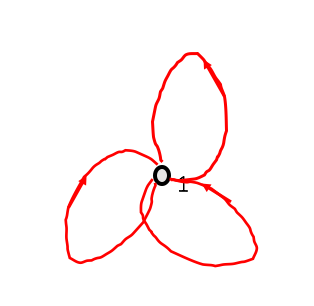
\includegraphics[width=0.25\textwidth]{week14/f_22}
\end{figure}
\item
Let $V=\{e_1,e_2,e_3\}$ and $E=\{e_1,\dots,e_6\}$, and define 
\[
\begin{array}{lll}
\delta(e_1)=(1,1),&
\delta(e_2)=(1,2),&
\delta(e_3)=(1,2),\\
\delta(e_4)=(2,3),&
\delta(e_5)=(2,3),&
\delta(e_6)=(3,3).
\end{array}
\]
The graph $(V,E)$ is represented below~(We do not care the direction of edges for this graph):
\begin{figure}[H]
\centering
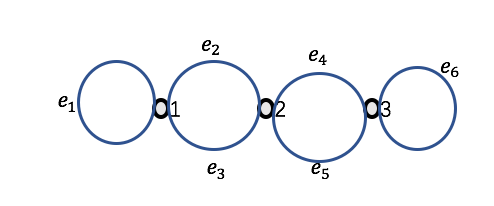
\includegraphics[width=0.3\textwidth]{week14/f_23}
\end{figure}
\end{enumerate}
\end{example}
\begin{definition}[Realizatin of a Graph]
For a given graph $\Gamma=(V,E)$, construct a realization by
\[
\{
|V|\times\{\text{zero simplies}\}
\coprod
|E|\times\{\text{$1$-simplies}\}
\}/\sim
\]
where the equivalence class is induced from the function $\delta$. 
We still call this realization of the graph as $\Gamma$.
\end{definition}


\begin{remark}
In general, graphs are not simplicial complexes.
But we can ``sub-divide'' each edge of $\Gamma$ into three parts such that there exists simplicial complex $K$ with $|K|\cong\Gamma$. For instance, 
\begin{figure}[H]
\centering
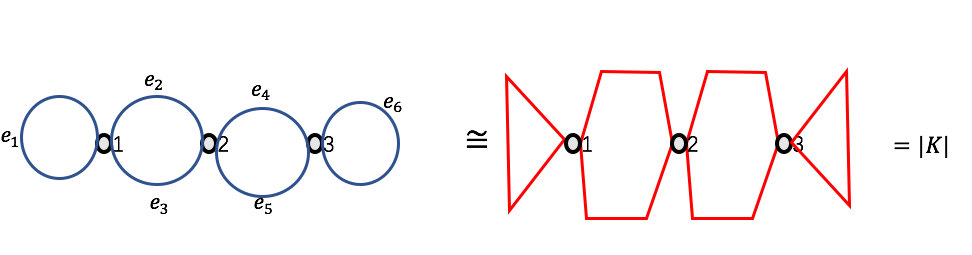
\includegraphics[width=\textwidth]{week14/f_24}
\end{figure}
where $|K|$ is a simplicial complex.
\end{remark}

\begin{definition}
\begin{itemize}
\item
Subgraph $\Gamma'\subseteq\Gamma$:
$\Gamma'=(V',E')$ with $V'\subseteq V$ and $E'\subseteq E$, and
\[
\delta\mid_{V'}:E'\to V'\times V'
\]
\item
Edge path:
A continous function $p:[0,1]\to\Gamma$ such that there exists $n\in\mathbb{N}$ satisfying
\[
p\mid_{[i/n,i+1/n]}:\left[\frac{i}{n},\frac{i+1}{n}\right]\to T
\]
is a path along an edge of $\Gamma$, or a constant function on a vertex of $\Gamma$, for $0\le i\le n-1$.
\begin{remark}
Under the homeomorphism $\Gamma\cong|K|$, each edge path is homotopic to $|g_\alpha|$ for some edge path $\alpha$ in the simplicial complex $K$.
For instance, 
\begin{figure}[H]
\centering
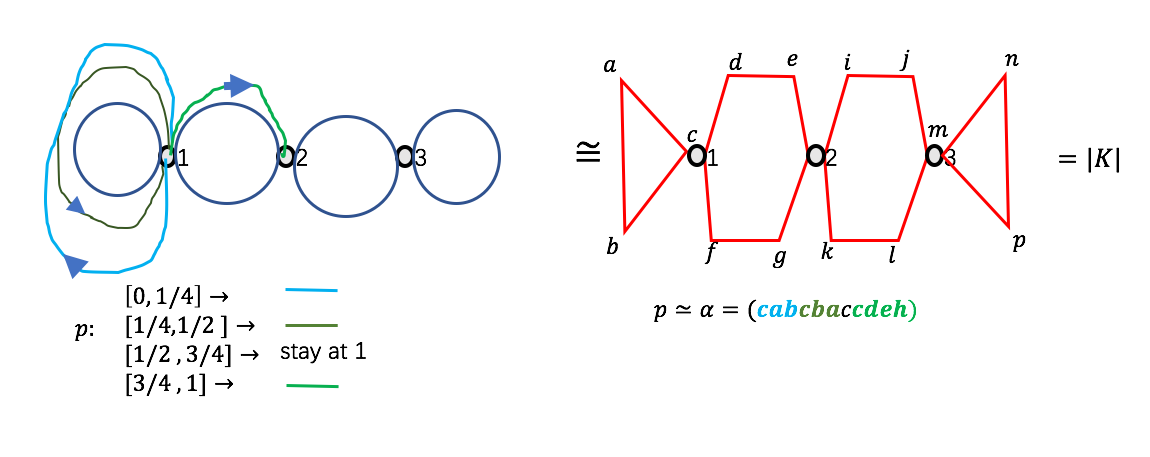
\includegraphics[width=\textwidth]{week14/f_26}
\end{figure}
\end{remark}
\item
An Edge loop is an edge path $p$ such that $p(0)=p(1)=b\in V$.
\item
Embedded Edge Loop: An injective edge loop, i.e., $p:[0,1]\to\Gamma$ such that 
\[
\text{for $x\notin V$},\quad
p^{-1}(x)=\emptyset\text{ or a single point}.
\]
\item
Tree: a connected graph $T$ that contains no embedded edge loop $p:[0,1]\to T$.

For instance, as shown in the figure, $T_1$ contains no edge loop, in particular, the edge loop $(a,b,a)$ is not embedded;
$T_2$ contains embedded edge loop $(a,b,c,d,a)$.
\item
Maximal Tree of a connected graph $\Gamma$:
\begin{itemize}
\item
A subgraph $T$ of $\Gamma$ such that $T$ is a tree.
\item
By adding an edge $e\in E(\Gamma)\setminus E(T)$ into $T$, the new graph is no longer a tree.
\end{itemize}
For instance, $T\subseteq\Gamma$ shown in the figure below is a maximal tree.
\begin{figure}[H]
\centering
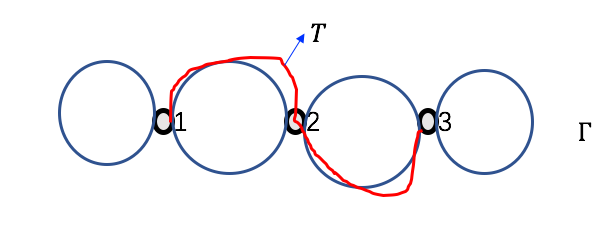
\includegraphics[width=0.5\textwidth]{week14/f_28}
\end{figure}
\end{itemize}
\end{definition}


\begin{theorem}
Let $\Gamma$ be a connected graph, and $T$ is a subgraph of $\Gamma$ such that $T$ is a tree.
Then $T$ is a maximal tree if and only if $V(T)=V(\Gamma)$.

Moreover, there always exists a maximal tree for all $\Gamma$.
\end{theorem}
\begin{proof}[Proof Outline for second part]
Construct an ordering of $\{v_1,\dots,v_i\}\subseteq V(\Gamma)$, such that for each integer $i\ge2$, 
there is an edge connecting $v_{i+1}$ with some vertex in $\{v_1,\dots,v_i\}$.

Then construct $T_1\subseteq T_2\subseteq\cdots$, where $T_i$ is a tree containing vertices $\{v_1,\dots,v_i\}$.
As a result, $T=\cup_{i\in\mathbb{N}}T_i$ is a maximal tree.
\end{proof}

\begin{theorem}
Let $\Gamma$ be a connected graph.
Then $\pi(\Gamma)$ is isomorphic to the free group generated by $\#\{E(\Gamma)\setminus E(T)\}$ elements,
for any maximal tree of $\Gamma$.
\end{theorem}

\begin{example}
\begin{enumerate}
\item
The graph $T\subseteq\Gamma_1$ shown in the figure below is a maximal tree.
\begin{figure}[H]
\centering
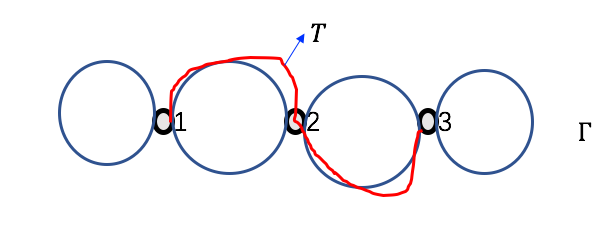
\includegraphics[width=0.45\textwidth]{week14/f_28}
\end{figure}
Therefore, $\pi_1(\Gamma_1)\cong\langle a,b,c,d\rangle$ since $\#\{E(\Gamma_1)\setminus E(T)\}=4$.
\item
The graph $T\subseteq\Gamma_2$ shown in the figure below is a maximal tree.
\begin{figure}[H]
\centering
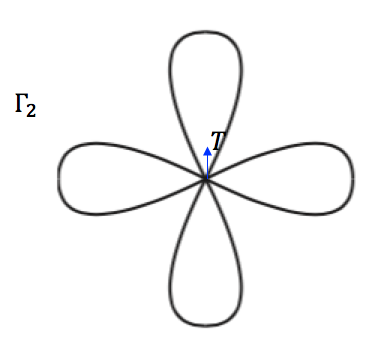
\includegraphics[width=0.25\textwidth]{week14/f_29}
\end{figure}
Therefore, $\pi_1(\Gamma_2)\cong\langle a,b,c,d\rangle$ since $\#\{E(\Gamma_2)\setminus E(T)\}=4$.
\item
Note that $\Gamma_1\simeq\Gamma_2$.
The reason for such homotopy equivalence is in the link
\[
\text{\url{https://www.math3ma.com/blog/clever-homotopy-equivalences}}
\]
\end{enumerate}
\end{example}















